\titre{}
\theme{equations}
\auteur{Nathan Scheinmann}
\niveau{1M}
\source{musy-2017}
\type{serie}
\piments{1}
\pts{}
\annee{2425}

\contenu{
	\tcblower
Complète les tableaux de valeurs ci-dessous à l'aide de la représentation graphique.
\begin{minipage}[t]{0.45\textwidth}{
\vspace{0pt}
	\begingroup
\renewcommand*{\arraystretch}{1.2}
	\begin{center}
\begin{tabular}{|c|c|c|c|c|c|c|}
	\hline
	\cellcolor{gray!40} $x$& $-3$ & $1$ &$-5$& \hspace{0.9cm}\phantom{t} &\hspace{0.9cm}\phantom{t} \\
	\hline
	\cellcolor{gray!40} $f(x)$&\hspace{0.9cm}\phantom{t}&\hspace{0.9cm}\phantom{t}&\hspace{0.9cm}\phantom{t}&$-2$&$1$\\
	\hline
\end{tabular}

\vspace{0.2cm}

\begin{tabular}{|c|c|c|c|c|c|c|}
	\hline
	\cellcolor{gray!40} $x$& $-5$ & $3$ &$0$& \hspace{0.9cm}\phantom{t} &\hspace{0.9cm}\phantom{t} \\
	\hline
	\cellcolor{gray!40} $g(x)$&\hspace{0.9cm}\phantom{t}&\hspace{0.9cm}\phantom{t}&\hspace{0.9cm}\phantom{t}&$-1$&$1$\\
	\hline
\end{tabular}

\vspace{0.2cm}

\begin{tabular}{|c|c|c|c|c|c|c|}
	\hline
	\cellcolor{gray!40} $x$& $1$ & $0$ &$-3$& \hspace{0.9cm}\phantom{t} &\hspace{0.9cm}\phantom{t} \\
	\hline
	\cellcolor{gray!40} $h(x)$&\hspace{0.9cm}\phantom{t}&\hspace{0.9cm}\phantom{t}&\hspace{0.9cm}\phantom{t}&$3$&$-5$\\
	\hline
\end{tabular}
\end{center}
\endgroup
}
\end{minipage}
\hfill
\begin{minipage}[t]{0.5\textwidth}{
\vspace{0pt}
\begin{center}
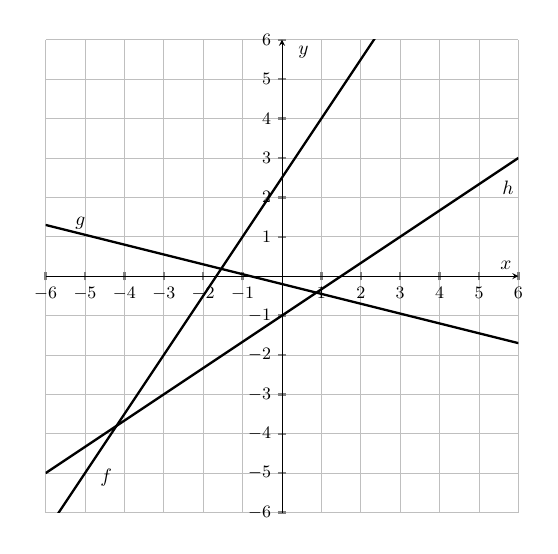
\begin{tikzpicture}[scale=0.7]
\begin{axis}[
  axis lines=center,
  grid=major,
  width=4in,
height=4in,
  xmin=-5,
  xmax=5,
  ymin=-5,
  ymax=5,
  xlabel=$x$,
  ylabel=$y$,
  enlargelimits={abs=1},
  xtick={-6,-5,...,6},
  ytick={-6,-5,...,6},
  xlabel style={at={(rel axis cs:1,0.5)}},
  ylabel style={at={(rel axis cs:0.52,1)}},
  tick style={very thick},
  ticklabel style={font=\small},
  legend style={
  at={(rel axis cs:1,1)},
  anchor=north west,
  draw=none,
  inner sep=0pt,
  fill=gray!10}
]

\addplot [very thick,domain=-6:6,samples=200] {2/3*x-1} node [below right,pos=0.95] {$h$};
%\addlegendentry {$f(x)=...$};
\addplot[black,very thick,domain=-6:6,samples=200]{3/2*x+2.5}  node[below right,pos=0.1] {$f$};
\addplot[black,very thick,domain=-6:6,samples=200]{-1/4*x-1/5}  node[above left,pos=0.1] {$g$};
%\addlegendentry{$g(x)=...$};
\end{axis}
\end{tikzpicture}
\end{center}	
}
\end{minipage}	

}
\correction{
	\tcblower
\begin{tasks}(2)
	\task premier tableau~: $-2;4;-5;-3;-1$
	\task deuxième tableau~: $1;-1;\simeq -0{,}2;3;-5$
	\task troisième tableau~: $\simeq -0{,}3;-1;-3;6;-6$
\end{tasks}
}

